\documentclass[10pt,conference]{IEEEtran}
\IEEEoverridecommandlockouts
\usepackage[spanish,es-tabla]{babel}
\renewcommand{\baselinestretch}{1.5}     %interlineado
\usepackage[utf8]{inputenc} 
\usepackage[square,numbers]{natbib}
\bibliographystyle{abbrvnat}
\usepackage{float}                      % para usar [H]
\usepackage[table,xcdraw]{xcolor}
\usepackage{amsmath,amssymb,amsfonts}
\usepackage{graphicx}
\usepackage{textcomp}
\usepackage{xcolor}
\usepackage{ragged2e} % \justify

%---------- pie de pagina
\usepackage{fancyhdr}
\pagestyle{fancy}
\fancyhf{}
\rfoot[]{\thepage}
%-----------------
\def\BibTeX{{\rm B\kern-.05em{\sc i\kern-.025em b}\kern-.08em
    T\kern-.1667em\lower.7ex\hbox{E}\kern-.125emX}}

\title{Árboles Binarios \\ {\Large Organización de Archivos}}
%--------------------------------------------
\author{
\IEEEauthorblockN{1\textsuperscript{do} Angely Mendez}
\IEEEauthorblockA{\textit{Escuela de Informática} \\
\textit{Universidad Nacional de Trujillo}\\
Trujillo, Perú \\
t052701020@unitru.edu.pe}
\and
\IEEEauthorblockN{2\textsuperscript{ero} Ciara Mendez}
\IEEEauthorblockA{\textit{Escuela de Informática} \\
\textit{Universidad Nacional de Trujillo}\\
Trujillo, Perú \\
t022700920@unitru.edu.pe}
}

%%--------------------------------------------
\begin{document}
\renewcommand{\IEEEkeywordsname}{{\bfseries Palabras claves:}} % Colocar Keywords en Spanish

\maketitle
%-------------------------------------------
\begin{abstract}
Este documento es una investigación e implementación en lenguaje C++ sobre árboles binarios que impone una estructura jerárquica sobre una colección de objetos. Ejemplos claros de utilización de árboles se presentan tanto dentro como fuera del área de computación (índices de libros, árboles genealógicos, etc.). En Informática constituyen una de las estructuras más utilizadas, con aplicaciones que van desde los árboles sintácticos, hasta la representación de datos que se desea mantener ordenados con un tiempo de acceso relativamente bajo. En general, se usarán árboles siempre que se quiera representar información jerarquizada, cuando esta converja en un solo punto. En este articulo se implementó las funciones que permiten la creación de registros a través de árboles binarios, en los que se puede escribir, mostrar, buscar, modificar, eliminar registros, ver los registros eliminados y hallar el máximo izquierdo de un registro. 
\end{abstract}

\begin{IEEEkeywords}
árboles binarios, árbol, informática, C++.
\end{IEEEkeywords}

\section{\textbf{Introducción}}
El árbol es una estructura de datos muy importante en informática y en ciencias de la computación. Los árboles son estructuras no lineales, al contrario que los arrays y las listas enlazadas que constituyen estructuras lineales. La estructura de datos árbol generaliza las estructuras lineales vistas en capítulos anteriores. Los árboles se utilizan para representar fórmulas algebraicas, para organizar objetos en orden de tal forma que las búsquedas son muy eficientes, y en aplicaciones diversas tales como inteligencia artificial o algoritmos de cifrado. Casi todos los sistemas operativos almacenan sus archivos en árboles o estructuras similares a árboles. Además de las aplicaciones citadas, los árboles se utilizan en diseño de compiladores, proceso de texto y algoritmos de búsqueda.
Entonces en este informe se presenta información al respecto, el cual está organizado de la siguiente manera: en primer lugar, se explican los conceptos teóricos: árboles generales, definiciones y terminología, luego se da énfasis en la implementación de las funciones en el lenguaje C++, para finalizar las conclusiones más relevantes.
%------------------------------------------
\section{\textbf{Árboles Binarios}} 
%\vspace{-22 mm}
\subsection{\textbf{Árboles Generales}}
Intuitivamente el concepto de árbol implica una estructura en la que los datos se organizan de modo que los elementos de información están relacionados entre sí a través de ramas. El árbol genealógico es el ejemplo típico más representativo del concepto de árbol general. La Figura~\ref{festruc} se representa un ejemplo de árbol general, gráficamente puede verse cómo un árbol invertido, la raíz en la parte más alta de la que salen ramas que llegan a las hojas, que están en la parte baja.
Un árbol consta de un conjunto finito de elementos, denominados nodos y un conjunto finito de líneas dirigidas, denominadas ramas, que conectan los nodos. El número de ramas asociado con un nodo es el grado del nodo.
\begin{figure}[H]
\begin{center}
       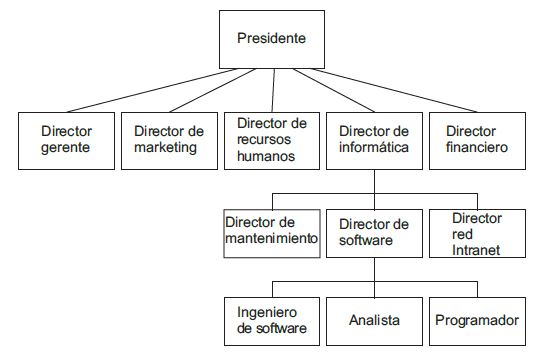
\includegraphics[width=8cm, height=5cm]{figuras/Arboljerar.JPG}
      \caption{Estructura Jerárquica tipo árbol}
      \label{festruc} 
      \end{center}
\end{figure}
\subsection{\textbf{Definición}}

Según a \citep{joyanes},Un árbol binario es un árbol en el que ningún nodo puede tener más de dos subárboles. En un árbol binario, cada nodo puede tener, cero, uno o dos hijos (subárboles). Se conoce el nodo
de la izquierda como hijo izquierdo y el nodo de la derecha como hijo derecho.

\par De acuerdo a \citep{ny}, un árbol consiste en un conjunto finito de elementos llamados nodos, o vértices y un conjunto finito de arcos dirigidos que conectan pares de nodos. Si el árbol no es vacío, entonces uno de los nodos, llamado la raíz, no tiene arcos entrantes, pero cualquier otro nodo en el árbol puede ser alcanzado desde él siguiendo un camino único, que es una secuencia de arcos consecutivos.

\par Algo similar menciona \citep{wiki} que, en ciencias de la computación, un árbol binario es una estructura de datos en la cual cada nodo puede tener un hijo izquierdo y un hijo derecho. No pueden tener más de dos hijos (de ahí el nombre "binario"). Si algún hijo tiene como referencia a null, es decir que no almacena ningún dato, entonces este es llamado un nodo externo. En el caso contrario el hijo es llamado un nodo interno. Usos comunes de los árboles binarios son los árboles binarios de búsqueda, los montículos binarios y Codificación de Huffman.

\par También \citep{cairo} menciona que, los árboles son las estructuras de datos no lineales y dinámicas de datos más importantes del área de computación. Se define un árbol binario tipo T como una estructura homogenea, resultado de la concatenación de un elemento de tipo T, llamado raíz, con unos árboles binarios disjuntos, llamados subárbol izquierdo y subárbol derecho.
%------------------------------------------------------------
\subsection{\textbf{Terminología}}
Además de la raíz, existen muchos términos utilizados en la descripción de los atributos de un árbol. En la Figura ~\ref{farb}, el nodo A es el raíz. Utilizando el concepto de árboles genealógicos, un nodo puede ser considerado como padre si tiene nodos sucesores.
Estos nodos sucesores se llaman hijos. Por ejemplo, el nodo B es el padre de los hijos E y F. El padre de H es el nodo D. Un árbol puede representar diversas generaciones en la familia.
Los hijos de un nodo y los hijos de estos hijos se llaman descendientes y el padre y abuelos de un nodo son sus ascendientes. Por ejemplo, los nodos E, F, I y J son descendientes de B. Cada nodo no raíz tiene un único padre y cada padre tiene cero o más nodos hijos. Dos o más nodos con el mismo padre se llaman hermanos. Un nodo sin hijos, tales como E, I, J, G y H se llaman nodo hoja.
\begin{figure}[H]
    \begin{center}
       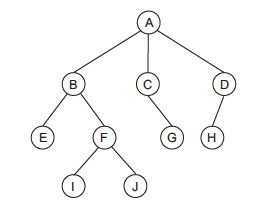
\includegraphics[width=8cm, height=5cm]{figuras/arbolgeneral.JPG}
      \caption{Árbol general}
      \label{farb} 
      \end{center}
\end{figure}
    
\begin{enumerate}[]
    \item {\textbf{Nivel:}}
    \par De acuerdo a \citep{gonzalez}, es la distancia al nodo raíz. La raíz tiene una distancia cero de sí misma, por ello se dice que la raíz está en el nivel 0. Los hijos del raíz están en el nivel 1, sus hijos están en el nivel 2 y así sucesivamente. Una cosa importante que se aprecia entre los niveles de nodos es la relación entre niveles y hermanos. Los hermanos están siempre al mismo nivel, pero no todos los nodos de un mismo nivel son necesariamente hermanos. Por ejemplo, en el nivel 2 (Figura ~\ref{farbter}), C y D son hermanos, al igual que lo son G, H, e I, pero D y G no son hermanos ya que ellos tienen diferentes padres.
    \item {\textbf{Camino:}}
    \par \citep{jorgeestructuras} Jorge Santiago menciona que, es una secuencia de nodos en los que cada nodo es adyacente al siguiente. Cada nodo del árbol puede ser alcanzado (se llega a él) siguiendo un único camino que comienza en el raíz. En la Figura ~\ref{farbter}, el camino desde el raíz a la hoja I, se representa por AFI. Incluye dos ramas distintas AF y FI.
    \item {\textbf{Altura o profundidad:}}
    \par Según \citep{pera}, es el nivel de la hoja del camino más largo desde la raíz más uno. Por definición1 la altura de un árbol vacío es 0. La Figura ~\ref{farbter} contiene nodos en tres niveles: 0, 1 y 2. Su altura es 3.
    \begin{figure}[H]
    \begin{center}
       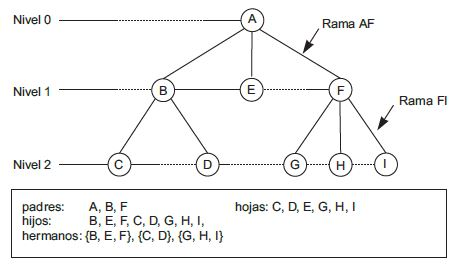
\includegraphics[width=8cm, height=5cm]{figuras/terminologia.JPG}
      \caption{Terminología de árboles}
      \label{farbter} 
      \end{center}
    \end{figure}
\end{enumerate}

%---------------------------------------------------------------------------
\section{\textbf{Implementación de las Funciones para el Árbol Binario en C++}} 
Para la implementación del Árbol Binario hemos considerado realizar un registro de datos personales de una persona, así que los siguientes códigos se basan en ello.
\begin{enumerate}[]
    \item {\textbf{Estructura Encabezado:}}
        \par Para definir el encabezado, ver Figura ~\ref{fencabeza}, se usó \textbf{struct} para poder almacenar varios campos, en este caso \textbf{NRS} que es la variable que almacena el número total de registros, \textbf{RZ} que significa la raíz del árbol y \textbf{URE} que es la variable que almacena el último registro eliminado, además la variable \textbf{e}.
        
        \begin{figure}[H]
            \begin{center}
            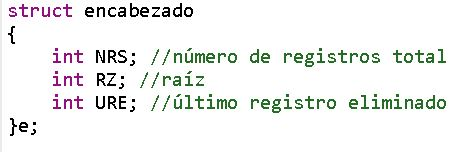
\includegraphics[width=7cm, height=2cm]{figuras/encabezado.JPG}
            \caption{Estructura Encabezado}
            \label{fencabeza} 
            \end{center}
        \end{figure}
        
    \item {\textbf{Estructura Person:}}
        \par Para definir el registro, obsérvese en la Figura ~\ref{fperson}, se usó \textbf{struct} para poder almacenar varios campos, en este caso los datos personales de una persona y usamos: \textbf{NR} que es la variable que almacena el número de registro, el campo \textbf{nombre} que es la variable que almacena el nombre, el campo \textbf{apellido} que es la variable que almacena el apellido,  el campo \textbf{celular} que es la variable que almacena el celular, el campo \textbf{email} que es la variable que almacena el correo electrónico, el campo \textbf{PI} que es la variable que almacena el puntero a la izquierda o rama izquierda del árbol, , el campo \textbf{PD} que es la variable que almacena el puntero a la derecha o rama derecha del árbol, el campo \textbf{ARE} que es la variable que almacena el anterior registro eliminado y además de los punteros \textbf{r}, \textbf{s} y \textbf{re max izq}.
        
        \begin{figure}[H]
            \begin{center}
            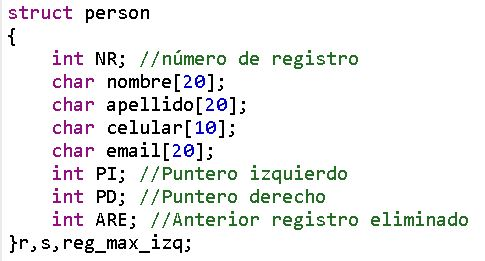
\includegraphics[width=8cm, height=3.5cm]{figuras/person.JPG}
            \caption{Estructura person}
             \label{fperson} 
             \end{center}
        \end{figure}
      
    \item {\textbf{Escribir:}}
       
         \begin{figure}[H]
            \begin{center}
            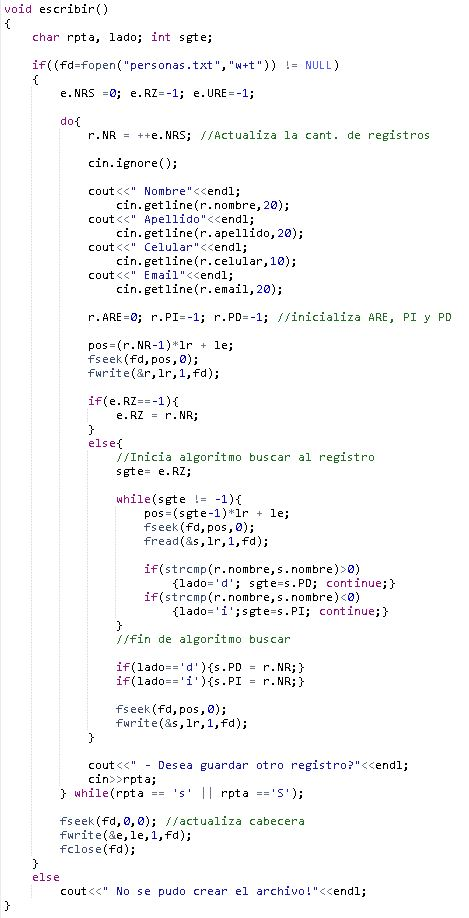
\includegraphics[width=8.5cm, height=16cm]{figuras/escribir.JPG}
            \caption{Función Escribir}
             \label{fescribir} 
             \end{center}
        \end{figure}
        
        \par En la función escribir, obsérvese en la Figura ~\ref{fescribir}, inicialmente se abre el archivo, es decir para ser escrito; además se inicializa la variable e en sus campos NRS, RZ y URE; que representa numero total de registros existentes, la rzia y el último registro eliminado respectivamente en el archivo.
        
        Dentro de un do while, incrementa en uno el NR del registro con el valor de NRS; se solicita ingresar al usuario la información de los campos para cada registro. Luego inicializa la variable r en sus campos ARE, PI, PD con 0 y los dos últimos con -1, que representa que no apuntan a ningún registro. Posteriormente posiciona y escribe en el registro con \textbf{fseek y fwrite}.
        
        Para el condicional, evalúa si la raíz es igual a $-1$, entonces la raiz es igual a número de registro. Por el contrario para el else, se emplea el algoritmo buscar al registro donde a la variable $sgte$ se le asigna el valor de la raiz, dentro del while calcula la posición de la variable sgte la posiciona y lee con fread.
        Además, evalúa donde irá almacenado, si al lado derecho o izquierdo. Por lo que, si el nombre ingresado es mayor irá al lado izquierdo de lo contrario al lado derecho.
        Luego actualiza los PD y PI de la variable s; según lo que la variable lado almacenó. Posiciona y escribe en el archivo.

        Para el do while mencionado inicialmente, seguirá ejecutándose si rpta es S o s, de no cumplirse se termina. Finalmente se actualiza el encabezado y cierra del archivo.
        
    \item {\textbf{Mostrar:}}
        \begin{figure}[H]
            \begin{center}
            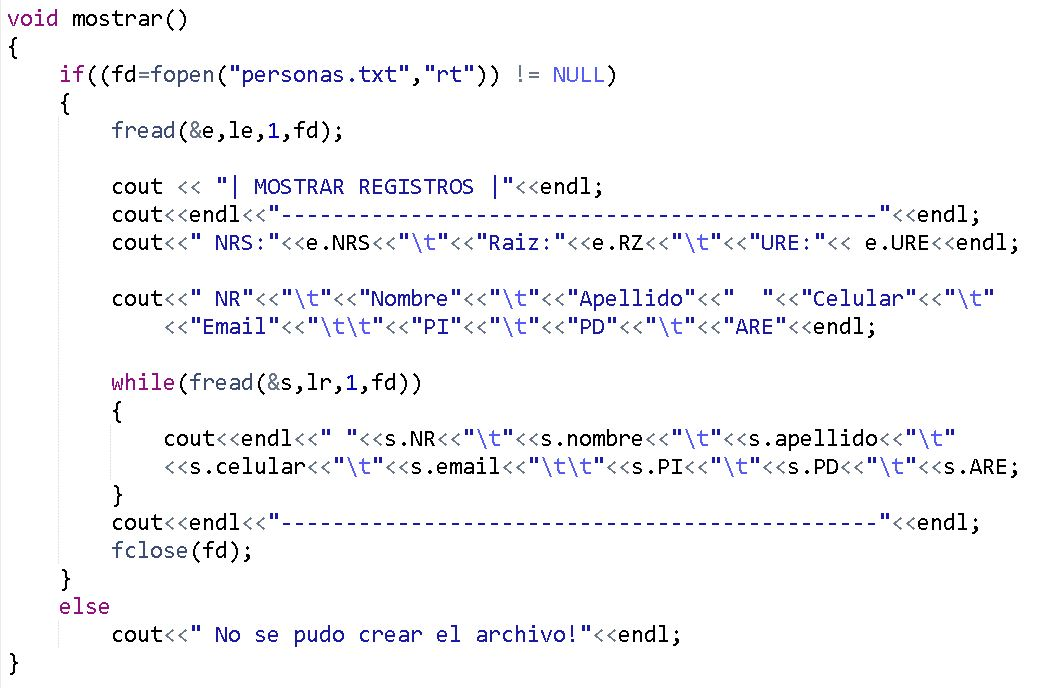
\includegraphics[width=8.5cm, height=5.5cm]{figuras/mostrar.JPG}
            \caption{Función Mostrar}
             \label{fmostrar} 
             \end{center}
        \end{figure}
        
         \par Para definir la función mostrar, ver Figura ~\ref{fmostrar}, primero, se abre el archivo $personas.txt$, luego, a través de \textbf{fread} se lee el encabezado para mostrar datos convenientemente y mediante un $while$, también se lee los datos a mostrar en pantalla, finalmente se cierra el archivo.
     
    \item {\textbf{Buscar:}}
        \par En la función buscar, obsérvese en la Figura ~\ref{fbuscar}, inicialmente se abre el archivo $personas.txt$, luego, a través de \textbf{fread}, se lee el encabezado; luego se solicita digitar al usuario el nombre que desea buscar. Después asignamos a la variable sgte, la raíz del árbol. Para recorrer todos los registros e ir buscando el nombre solicitado usamos un $while$, se calcula la posición de $sgte$, se lee el archivo y a través de if, comparamos hasta que encontrar el nombre solicitado, mientras se va actualizando la variable $sgte$ a los punteros: izquierda o derecha, cuando se encuentra el nombre ingresado, se muestra los datos en el registro del árbol de esa persona. También se actualiza la variable $band$, de lo contrario se mostraría el mensaje: El nombre no existe.
        %\vspace{-5 mm}
        
         \begin{figure}[H]
            \begin{center}
            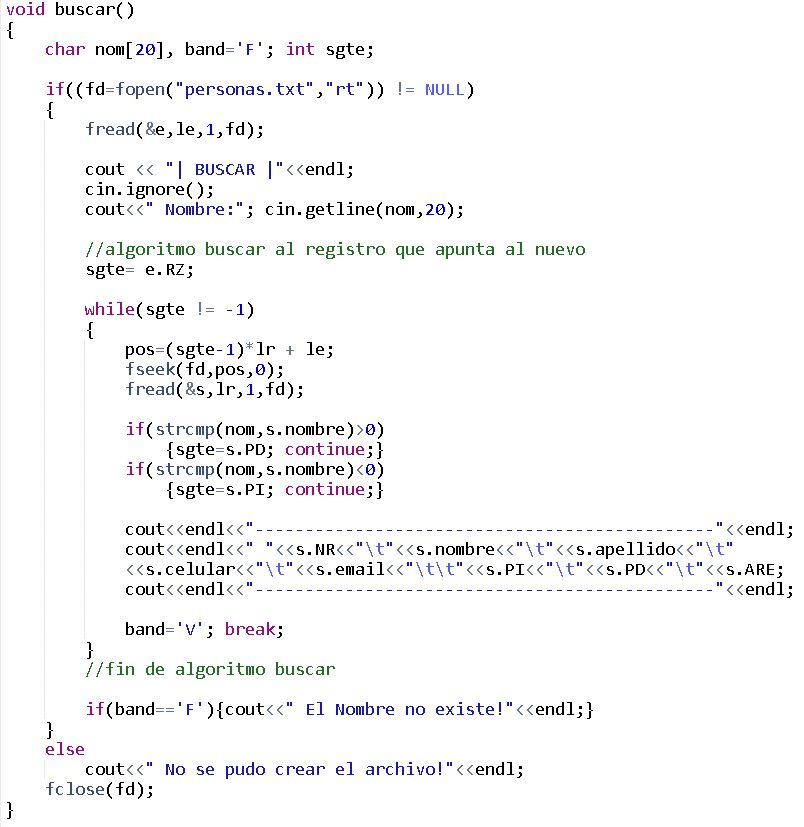
\includegraphics[width=8.5cm, height=10cm]{figuras/buscar.JPG}
            \caption{Función Buscar}
             \label{fbuscar} 
             \end{center}
        \end{figure}
  
    \item {\textbf{Insertar:}}
        \par En esta función, ver Figura ~\ref{finsertar}, es de manera similar que la función escribir, solo que aquí se \textbf{evita la inicialización del campo NRS, RZ, URE} en la variable e; porque esos son campos globales y puede existir la posibilidad que ya existan registros, por lo que si las inicializamos nuestro programa no funcionará y no almacenara los registros de manera adecuada, debido a que en ese campo se inicializa en 0. Luego todo es exactamente igual que la función escribir.
        
        \begin{figure}[H]
            \begin{center}
            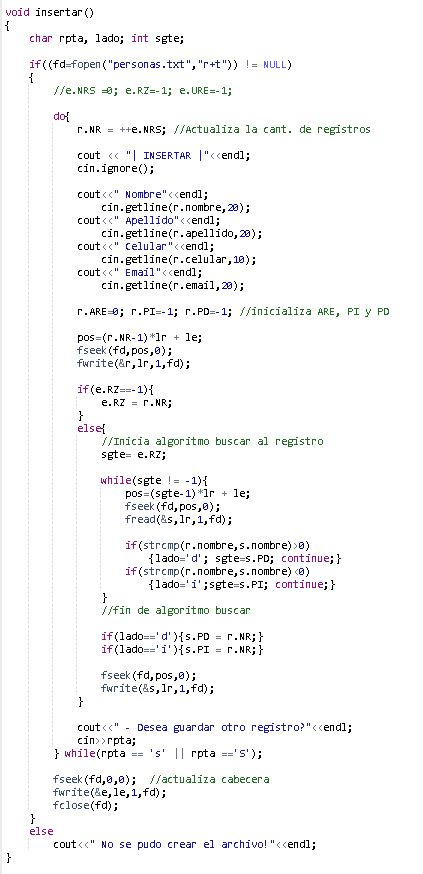
\includegraphics[width=8.5cm, height=13cm]{figuras/insertar.JPG}
            \caption{Función Insertar}
             \label{finsertar} 
             \end{center}
        \end{figure}
    
    \item {\textbf{Modificar Celular:}}
        \par En la función modificar, ver Figura ~\ref{fmodificar}, inicialmente se abre el archivo para ser modificado $r + t$, es decir para poder leer y escribir, \textbf{personas.txt}, luego con \textbf{fread}, se lee el encabezado y se solicita digitar al usuario el nombre que desea modificar.
        
        Después, a través del while como primer paso, se \textbf{busca en los registros} realizándose comparaciones, actualizando a su vez los punteros: izquierda y derecha, de encontrarse se realiza el segundo paso donde \textbf{solicita digitar el nuevo Celular}, actualizando dicha información a través de posicionar y escribir, con \textbf{fseek y fwrite} en el registro, por otro lado, de no encontrarse el nombre muestra un mensaje. Finalmente actualiza el encabezado, y cierra el archivo.
        \begin{figure}[H]
            \begin{center}
            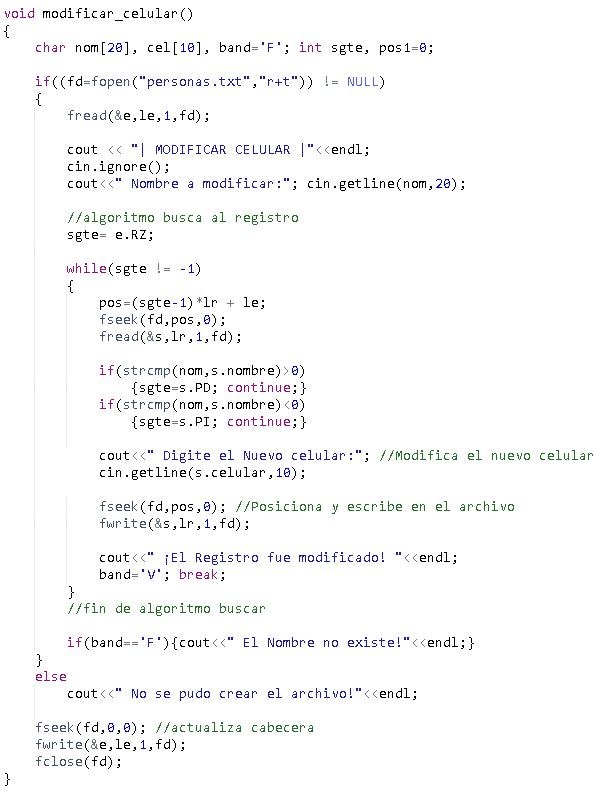
\includegraphics[width=8.5cm, height=10cm]{figuras/modificarcelular.JPG}
            \caption{Función Modificar}
             \label{fmodificar} 
             \end{center}
        \end{figure}
        
        
    \item {\textbf{Eliminar:}}
        
        \par Para la función eliminar, obsérvese en la Figura ~\ref{feliminar1}, se inicializan las variables locales que usará esta función; inicialmente se abre el archivo \textbf{personas.txt}, luego con fread, se lee el encabezado y se solicita digitar al usuario el nombre que desea eliminar.
        
        Después, a través del while como paso $0$, se \textbf{busca en los registros} realizándose comparaciones con el if, de encontrarse, actualiza la band con true.
        
        Y se evalúa para dos opciones si tiene máximo izquierdo y si no tiene máximo izquierdo.
        
        \begin{figure}[H]
            \begin{center}
            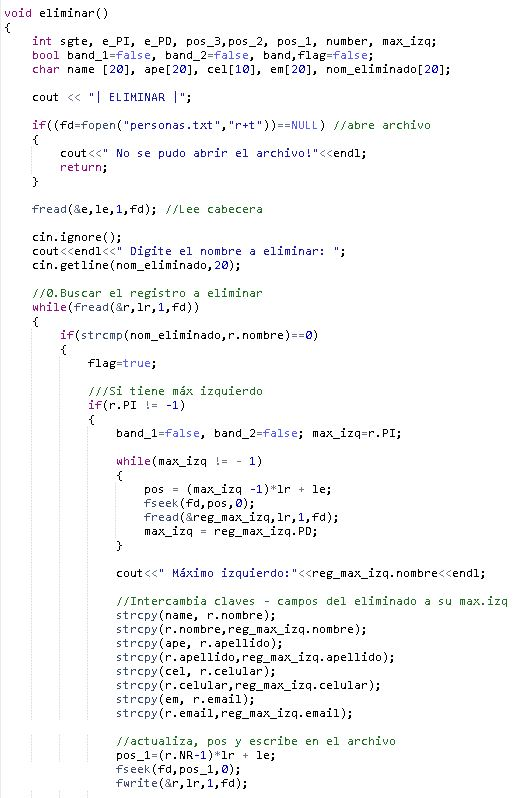
\includegraphics[width=8.5cm, height=10cm]{figuras/eliminar1.JPG}
            \caption{Función Eliminar - Primera parte}
             \label{feliminar1} 
             \end{center}
        \end{figure}
        Para el primer caso realiza la búsqueda con el while del máximo izquierdo, cuando lo encuentra intercambia las claves.
        
        Obsérvese en la Figura ~\ref{feliminar2}, aquí como se consideraron varios campos, se almacena en las variables name, ape, cel y em, la información del que será eliminado.
        
        Luego reemplaza los campos del eliminado con los del max.izq. Actualiza y escribe en el archivo lo realizado.
        
        Continua el intercambio de claves pero ahora los campos del máximo izquierdo a los campos del eliminado. Mediante un while recorre todo el registro y actualiza los campos. Además, actualiza el URE y ARE, almacenando los valores de los punteros PD y PI.
        
        En el siguiente while según el NR a eliminar se actualizan mediante condicionales los valores anteriormente almacenados de PI y PD.
        
        \begin{figure}[H]
            \begin{center}
            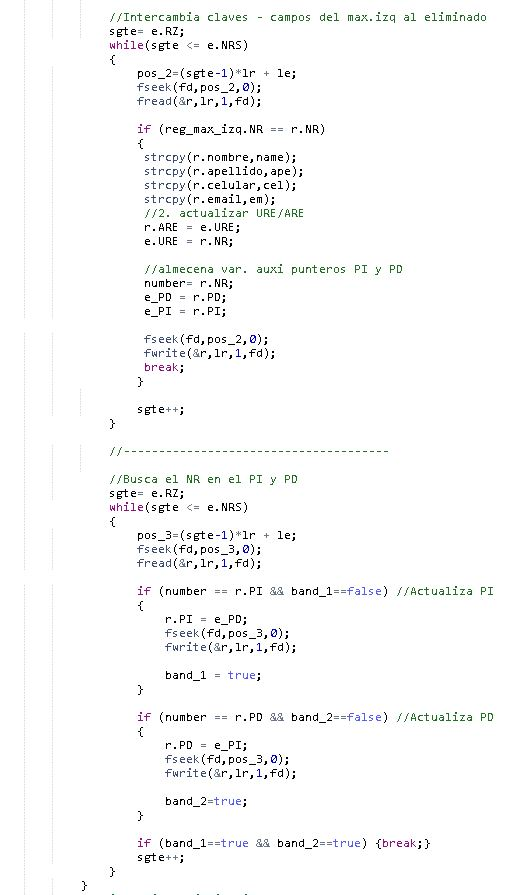
\includegraphics[width=8.5cm, height=10cm]{figuras/eliminar2.JPG}
            \caption{Función Eliminar - Segunda parte}
             \label{feliminar2} 
             \end{center}
        \end{figure}
        \begin{figure}[H]
            \begin{center}
            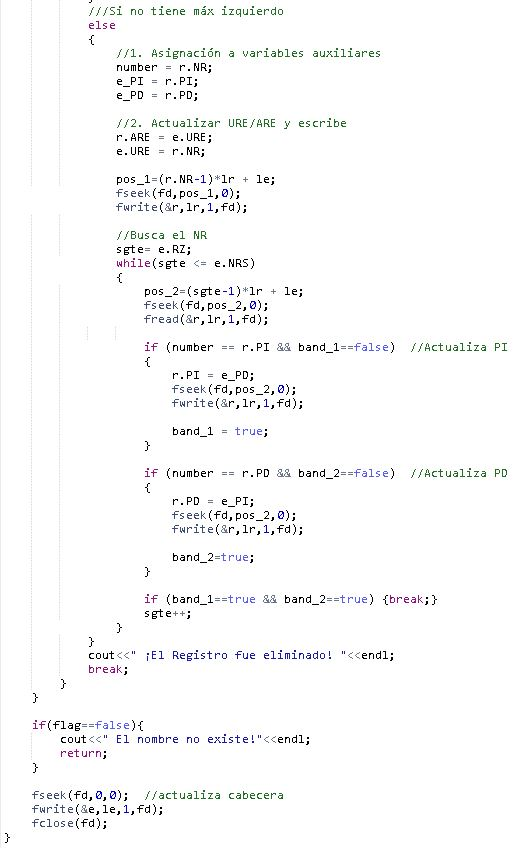
\includegraphics[width=8.5cm, height=10cm]{figuras/elimnar3.JPG}
            \caption{Función Eliminar - Tercera parte}
             \label{feliminar3} 
             \end{center}
        \end{figure}
        
        Para el segundo caso, donde no tiene máximo izquierdo, se asigna a variables auxiliares los valores de NR, PI y PD. Asimismo actualiza los valores de URE/ARE. Posicionando y escribiendo en el archivo.
        
        Y el siguiente while según el NR a eliminar se actualizan mediante condicionales los valores anteriormente almacenados de PI y PD.
        
        De cumplirse uno de los dos casos, muestra registro eliminado. Por otro lado, de no encontrarse el nombre muestra un mensaje. Finalmente posiciona y escribe con \textbf{fseek y fwrite} actualiza el encabezado, y cierra el archivo.
        
     \item {\textbf{Ver Eliminados:}}  
     \par Para definir la función Ver Eliminados, ver Figura ~\ref{fvereliminar}, primero, se abre el archivo $personas.txt$, luego, a través de \textbf{fread} se lee el encabezado para mostrar datos convenientemente, posteriormente asignamos a la variable $sgte$ el $URE$ y mediante un $while$ se recorre todo el árbol, actualizamos la $pos$ a través de \textbf{fseek} y se lee a través de \textbf{fread}, finalmente se lee los datos a mostrar en pantalla y se actualiza el $ARE$ en $sgte$, para terminar se cierra el archivo.
        \begin{figure}[H]
            \begin{center}
            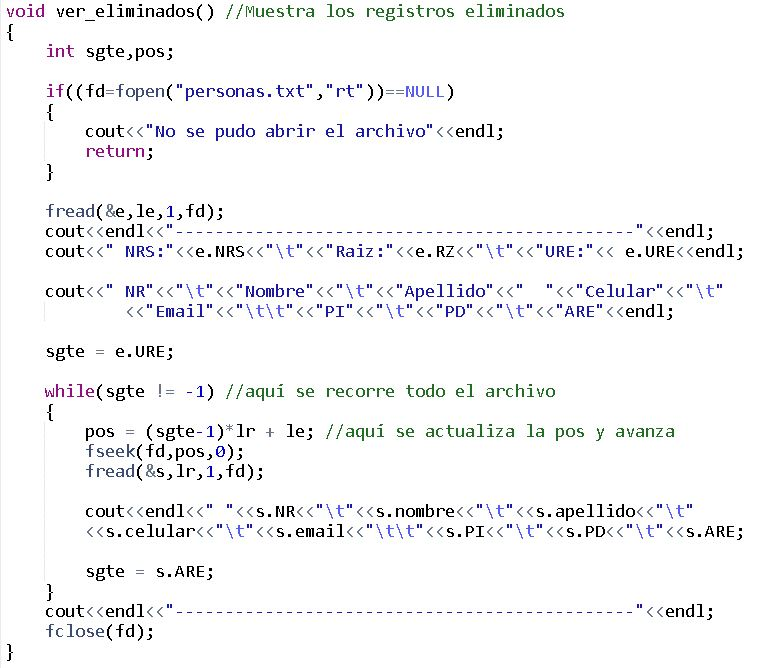
\includegraphics[width=8.5cm, height=7cm]{figuras/vereliminados.JPG}
            \caption{Ver eliminados}
             \label{fvereliminar} 
             \end{center}
        \end{figure}
        
     \item {\textbf{Máximo Izquierdo:}} 
     \par Para definir la función Máximo Izquierdo, ver Figura ~\ref{fmax}, primero, se abre el archivo $personas.txt$, luego, a través de \textbf{fread} se lee el encabezado. Luego, se pide al usuario digitar el nombre a buscar si tiene Máximo Izquierdo. Posteriormente asignamos a la variable $sgte$ el $RZ$ y mediante un $while$ se recorre todo el árbol, actualizamos la $pos$ a través de \textbf{fseek} y se lee a través de \textbf{fread}, para poder realizar las comparaciones usando $strcmp$, a su vez se va actualizando el valor de $sgte$ con los punteros: izquierdo y derecho, aquí se termina la búsqueda del nombre ingresado. Finalmente se calcula el Máximo Izquierdo, a través de un $while$ se recorre todo el árbol, se actualiza la pos y se leen datos. Para terminar, se muestra en pantalla el máximo izquierdo del nombre ingresado, de lo contrario que, el nombre no existe y se cierra el archivo.
       \begin{figure}[H]
            \begin{center}
            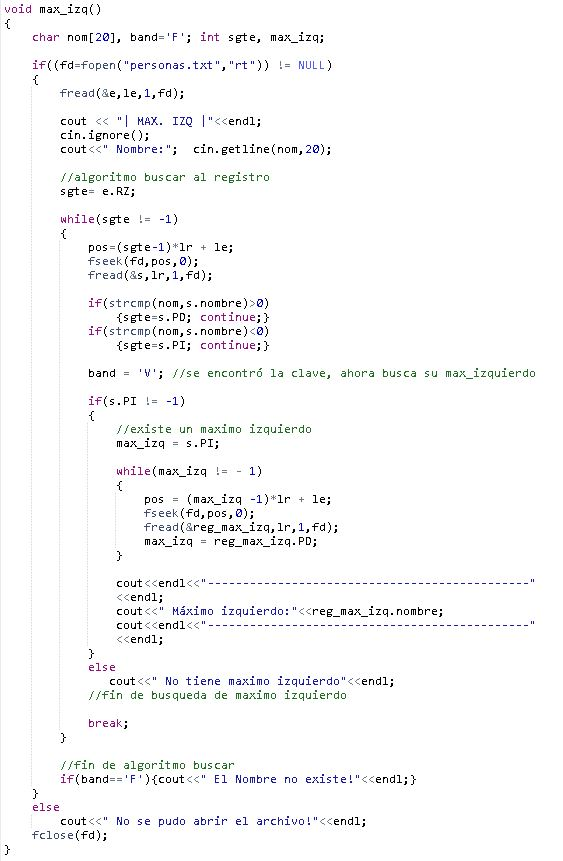
\includegraphics[width=8.5cm, height=11cm]{figuras/max_izqu.JPG}
            \caption{Función Máximo Izquierdo}
             \label{fmax} 
             \end{center}
        \end{figure}
\end{enumerate}

\section{\textbf{Conclusiones}}
Este informe presentó información relevante acerca de árboles binarios, se ha explicado los conceptos teóricos relacionados con este, cabe precisar que las ramas del árbol está representada por los campos PI y PD; las cuáles siempre tendrán un valor, pues son la base de la creación del árbol. Además de permitir conocer sobre la implementaciones de árboles binarios, con sus respectivas explicaciones, además de otras funciones que permiten la creación de registros y archivos, con extensión $*.txt$. en el que se puede escribir, mostrar, buscar, modificar, eliminar y ver registros eliminados, además encontrar el máximo izquierdo de un registro.

%-------------------------------------------------------
\medskip
\bibliography{refer}
\end{document}
